\documentclass{article}
\usepackage[utf8]{inputenc}
\usepackage{graphicx}
\usepackage{subfig}
\newpage
\newpage
\title{EC2017}
\author{Chetan sarigala }
\date{December 16, 2020}
\begin{document}
\maketitle
\begin{document}
\section{EC2017 44 }

  

         \begin{question}
            Figure I shows a 4-bit ripple carry adder realized using full adders and Figure II shows the circuit of a full-adder (FA). The propagation delay of the XOR, AND and OR gates in Figure II are 20 ns, 15 ns and 10 ns, respectively. Assume all the inputs to the 4-bit adder are initially reset to 0.
\begin{figure}[!ht]
\centerline{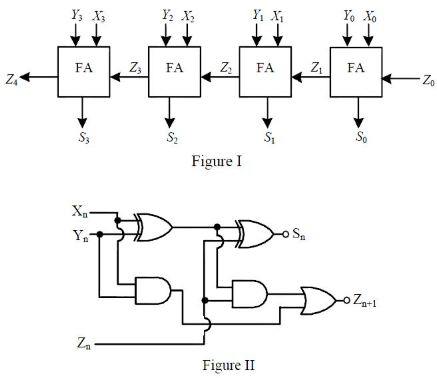
\includegraphics[scale=2.5]{Q-144.PNG}}
	
	\label{Q-144.PNG}
\end{figure}

At t = 0, the input to the 4-bit adder are changed to X3 X2 X1 Xo = 1100, Y3 Y2 Y1 Yo = 0100 and Zo = 1. The output of the ripple carry adder will be stable at t (in ns  )=____________



         \end{question}

         \begin{answer}
        \title {ANSWER} \begin{figure}[!ht]
    \centerline{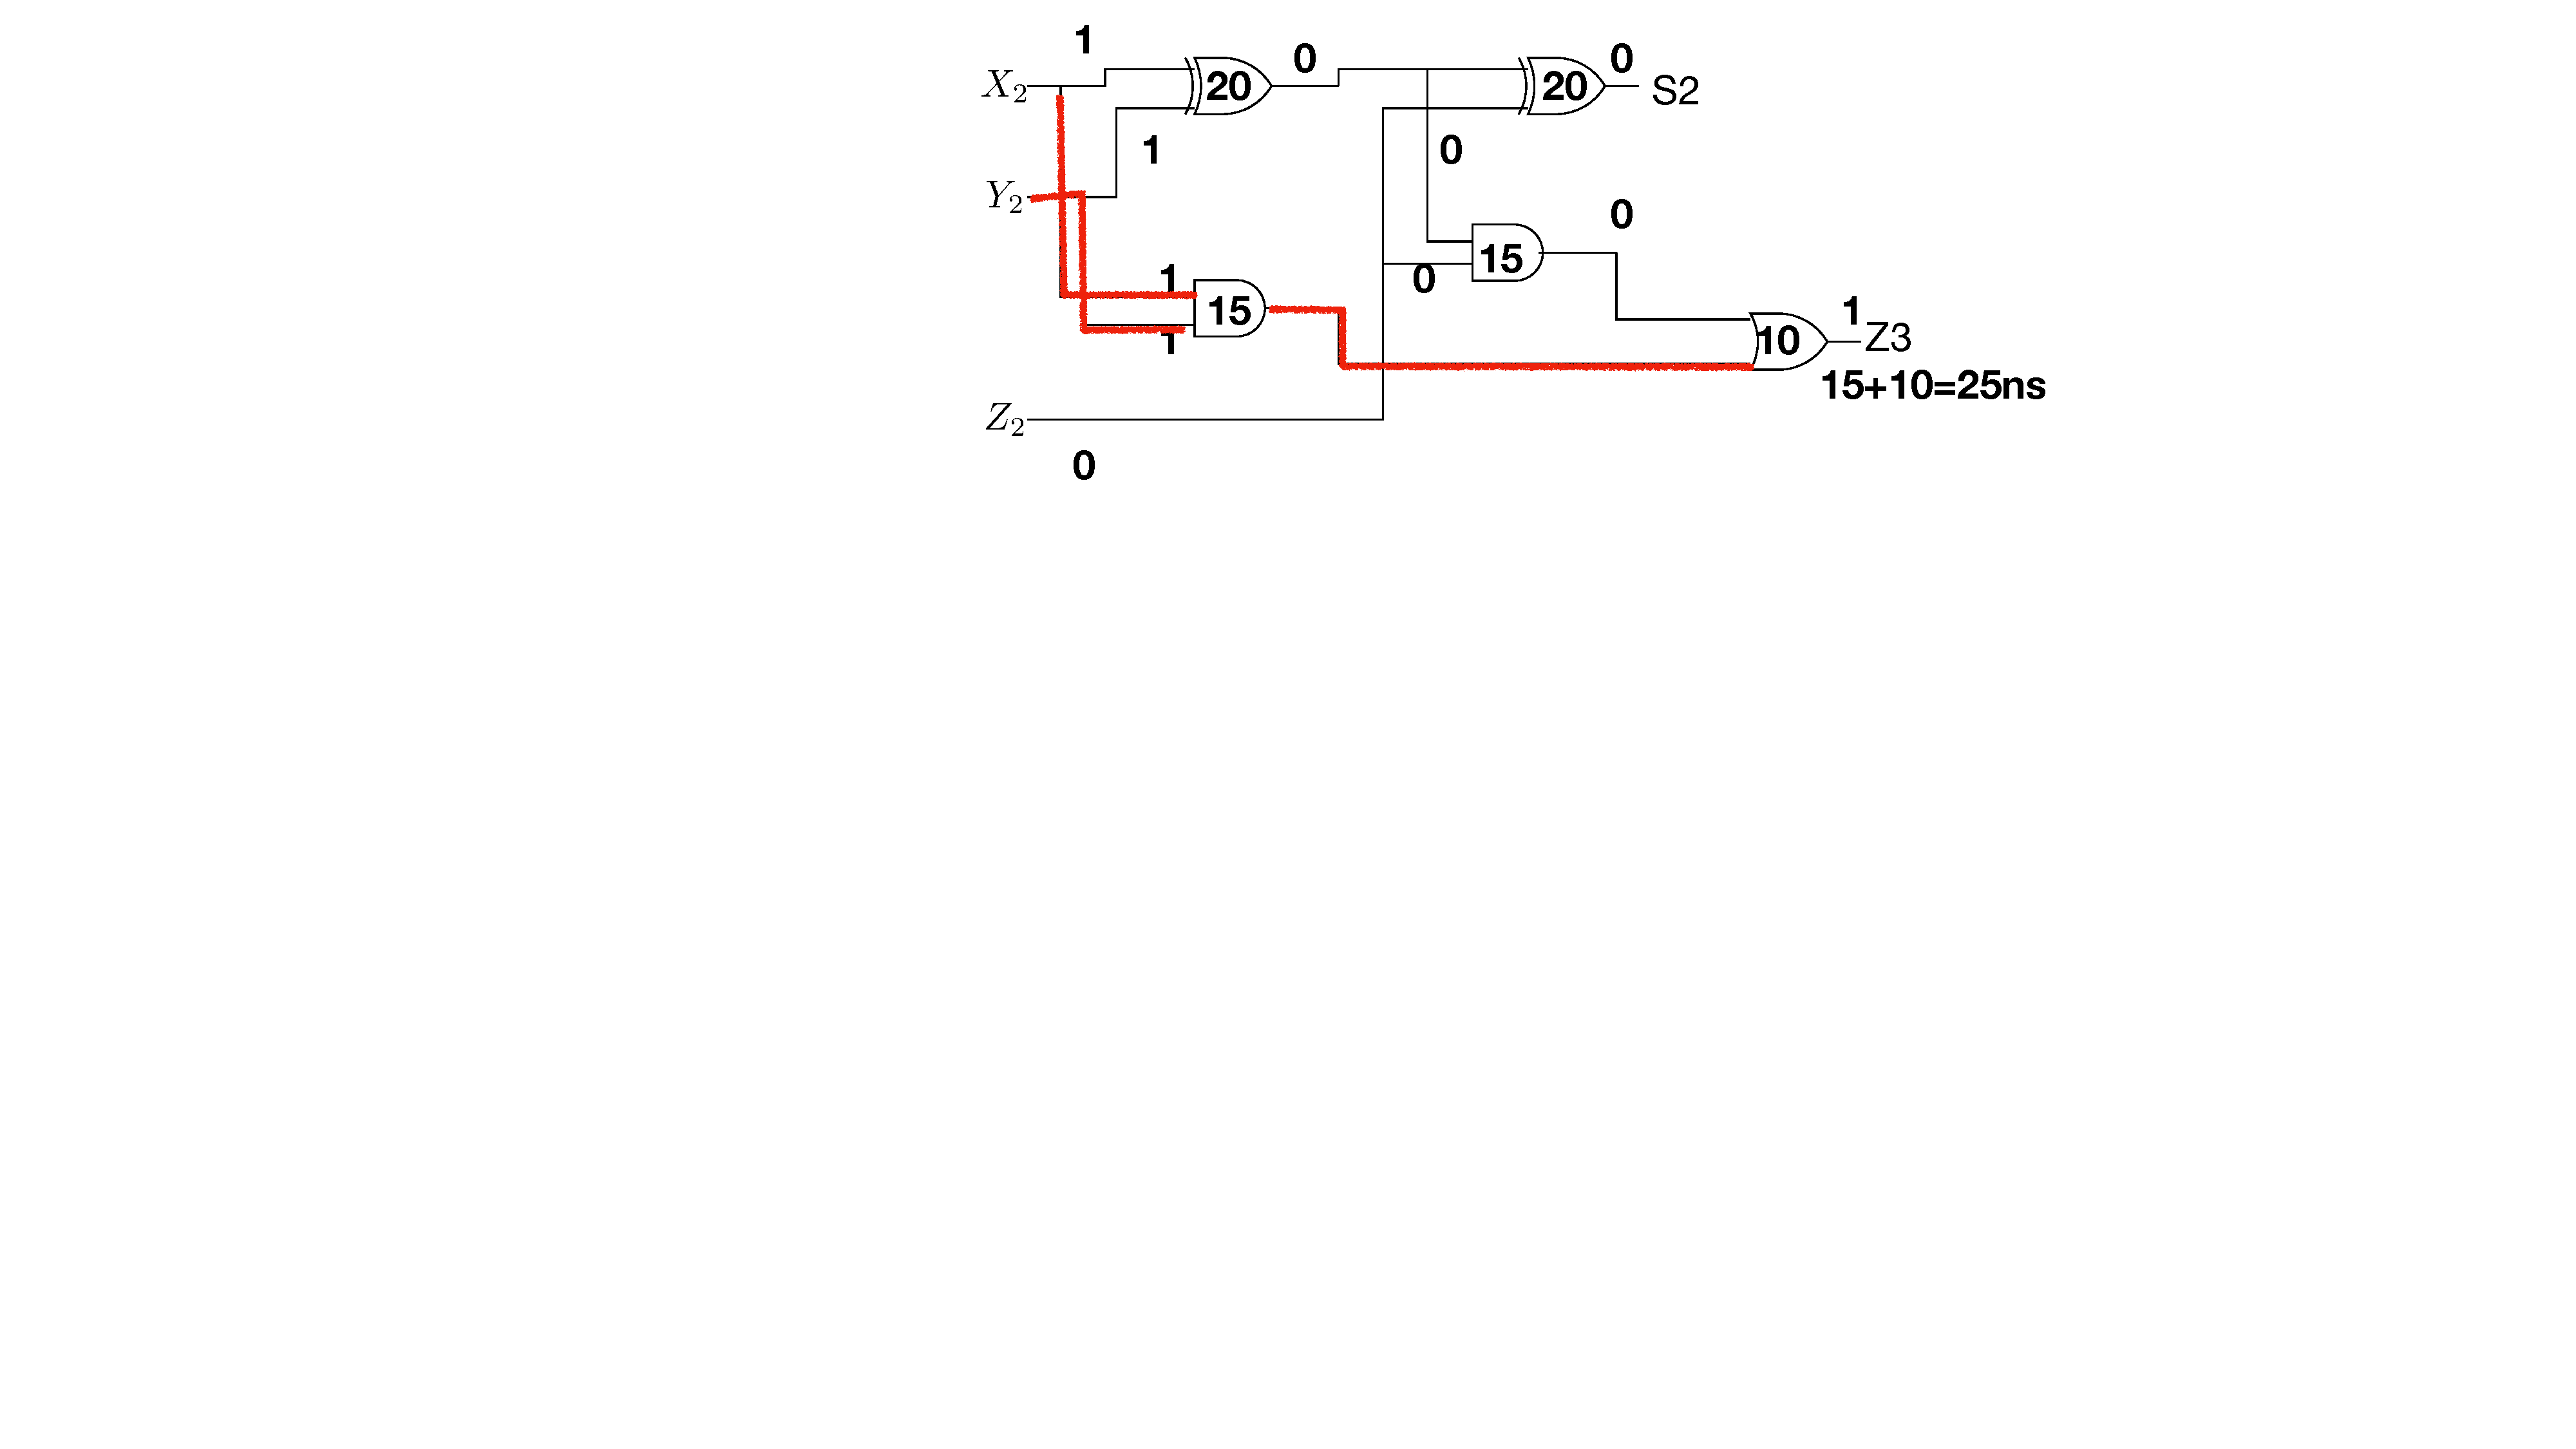
\includegraphics[scale=.5]{quad1.pdf}}
		\caption{}
	\label{quad1.pdf}
\end{figure}
        \bibliographystyle{}
   \begin{figure}[!ht]
    	\centerline{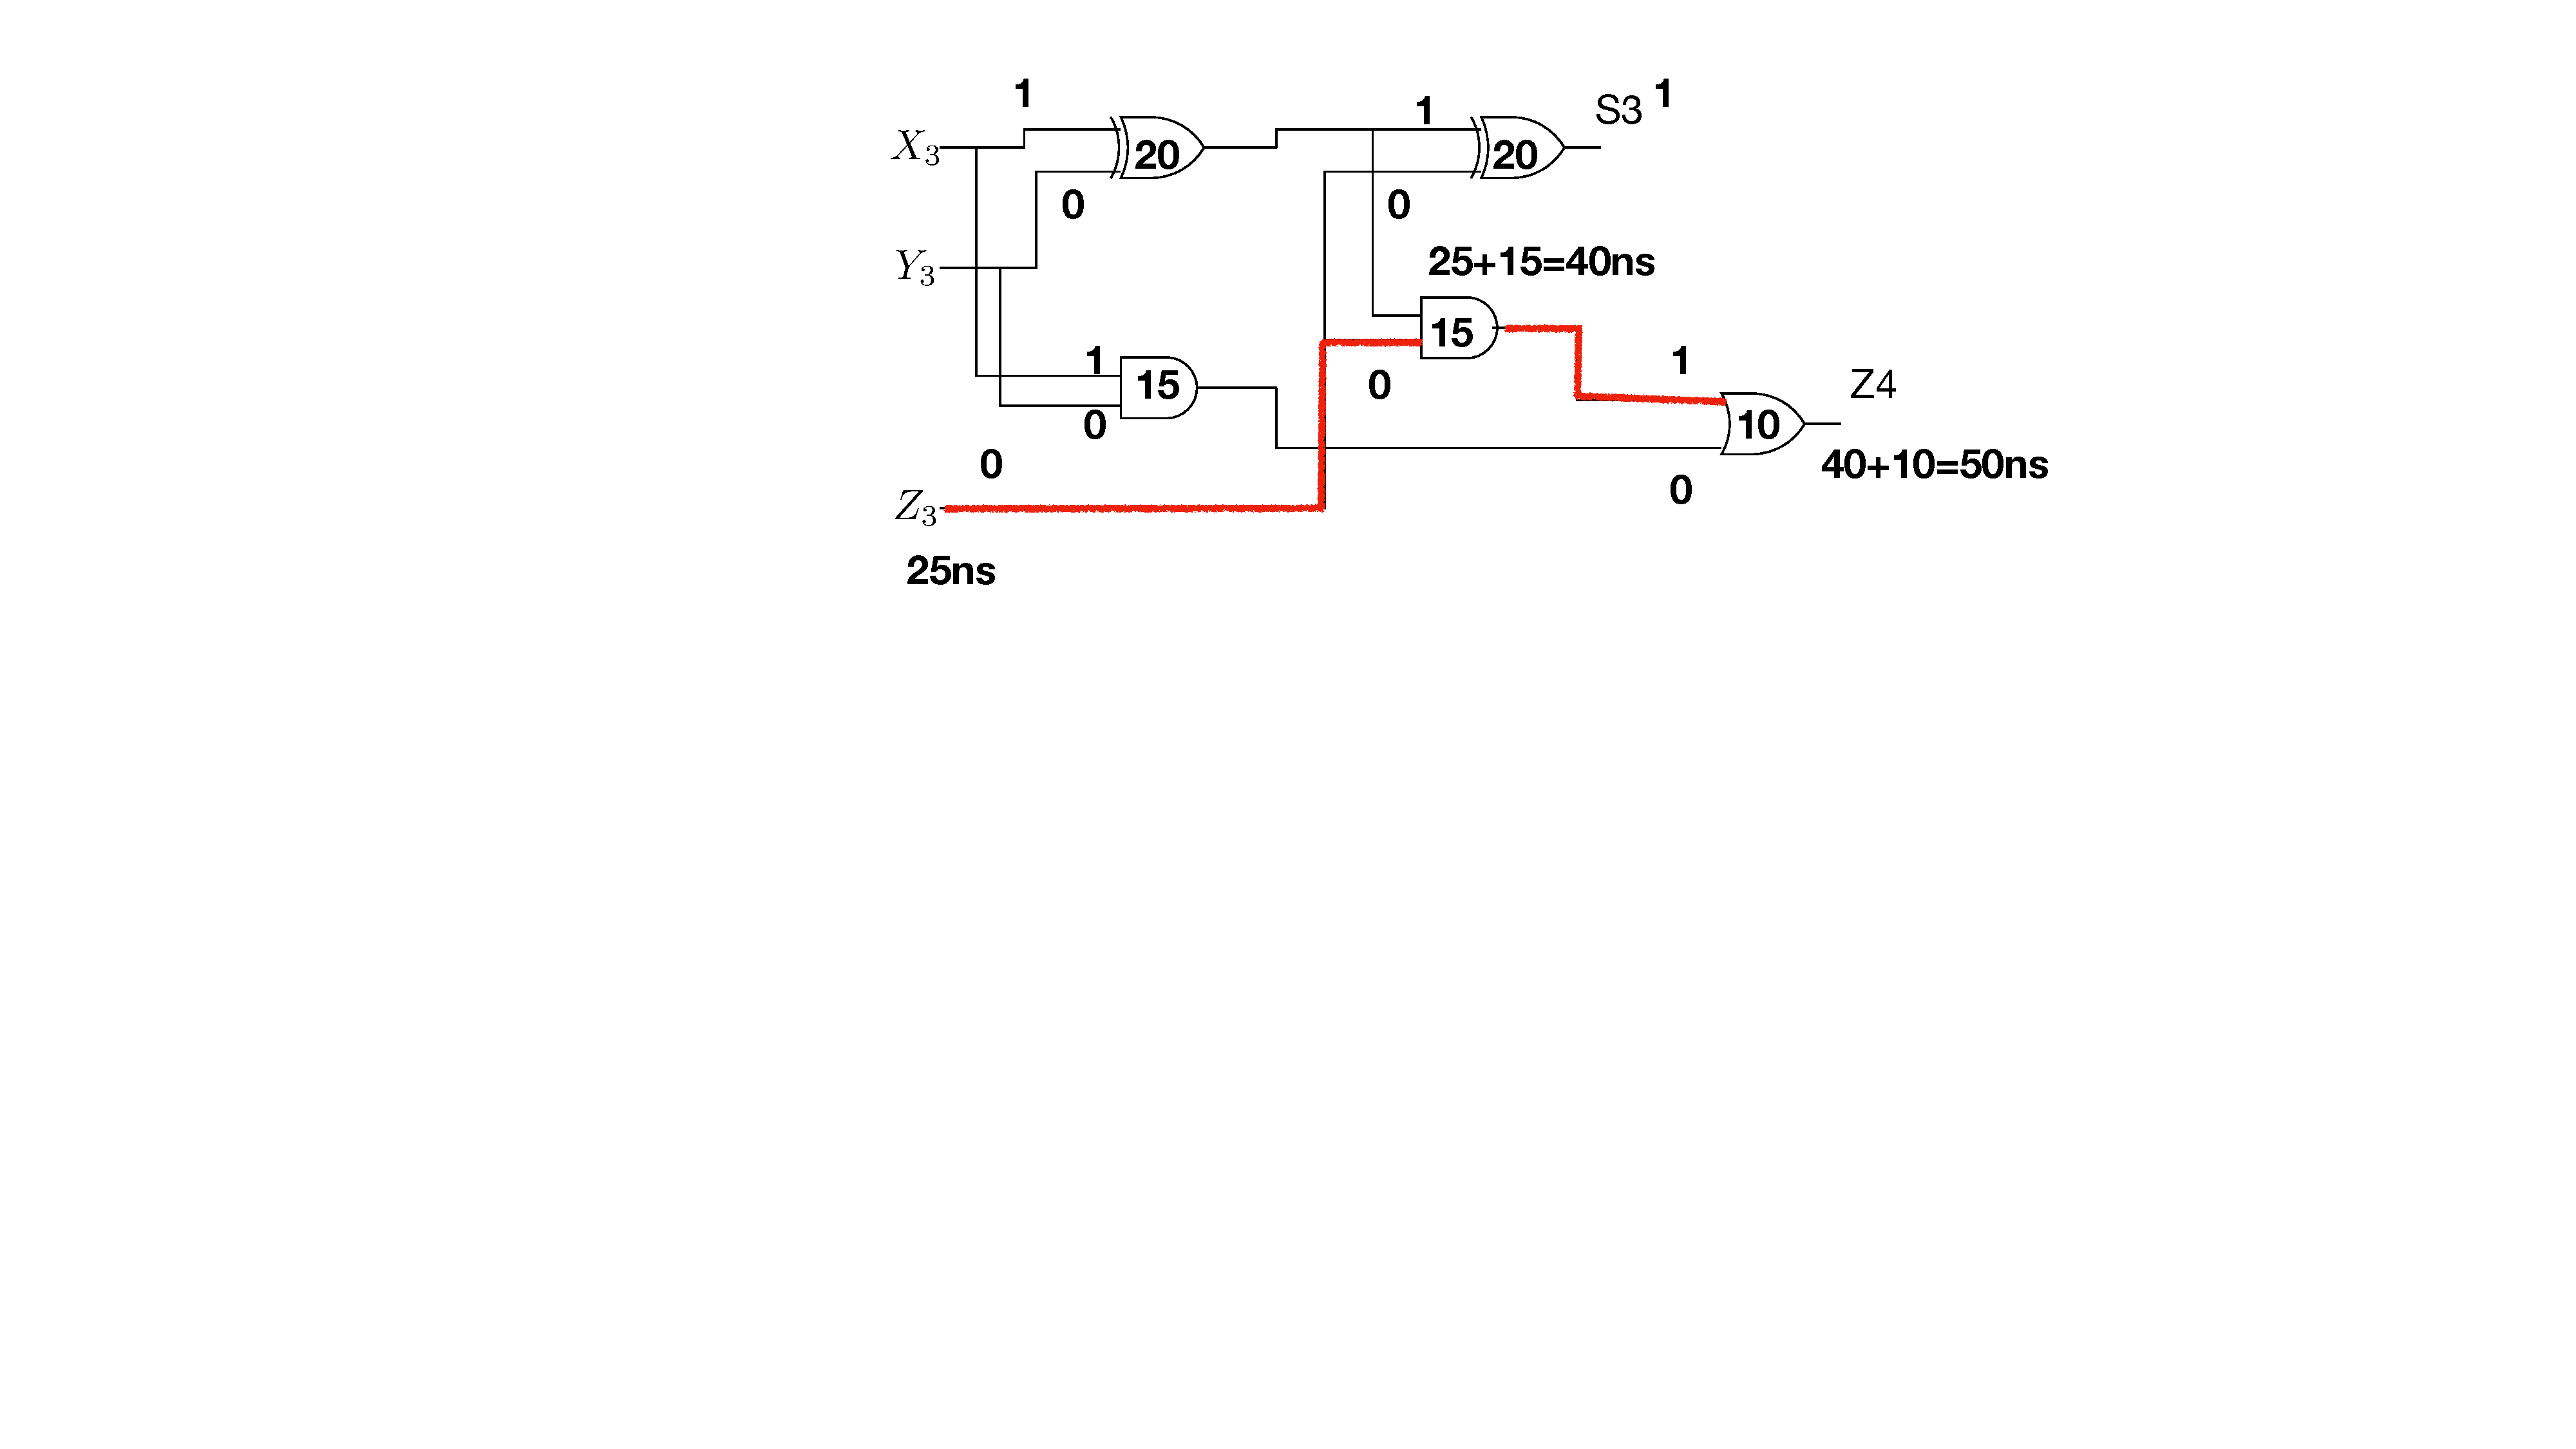
\includegraphics[scale=.5]{quad2.pdf}}
    	\caption{}
   
	
	\label{quad2.pdf}
\end{figure}
   	\begin{figure}[!ht]
    \centerline{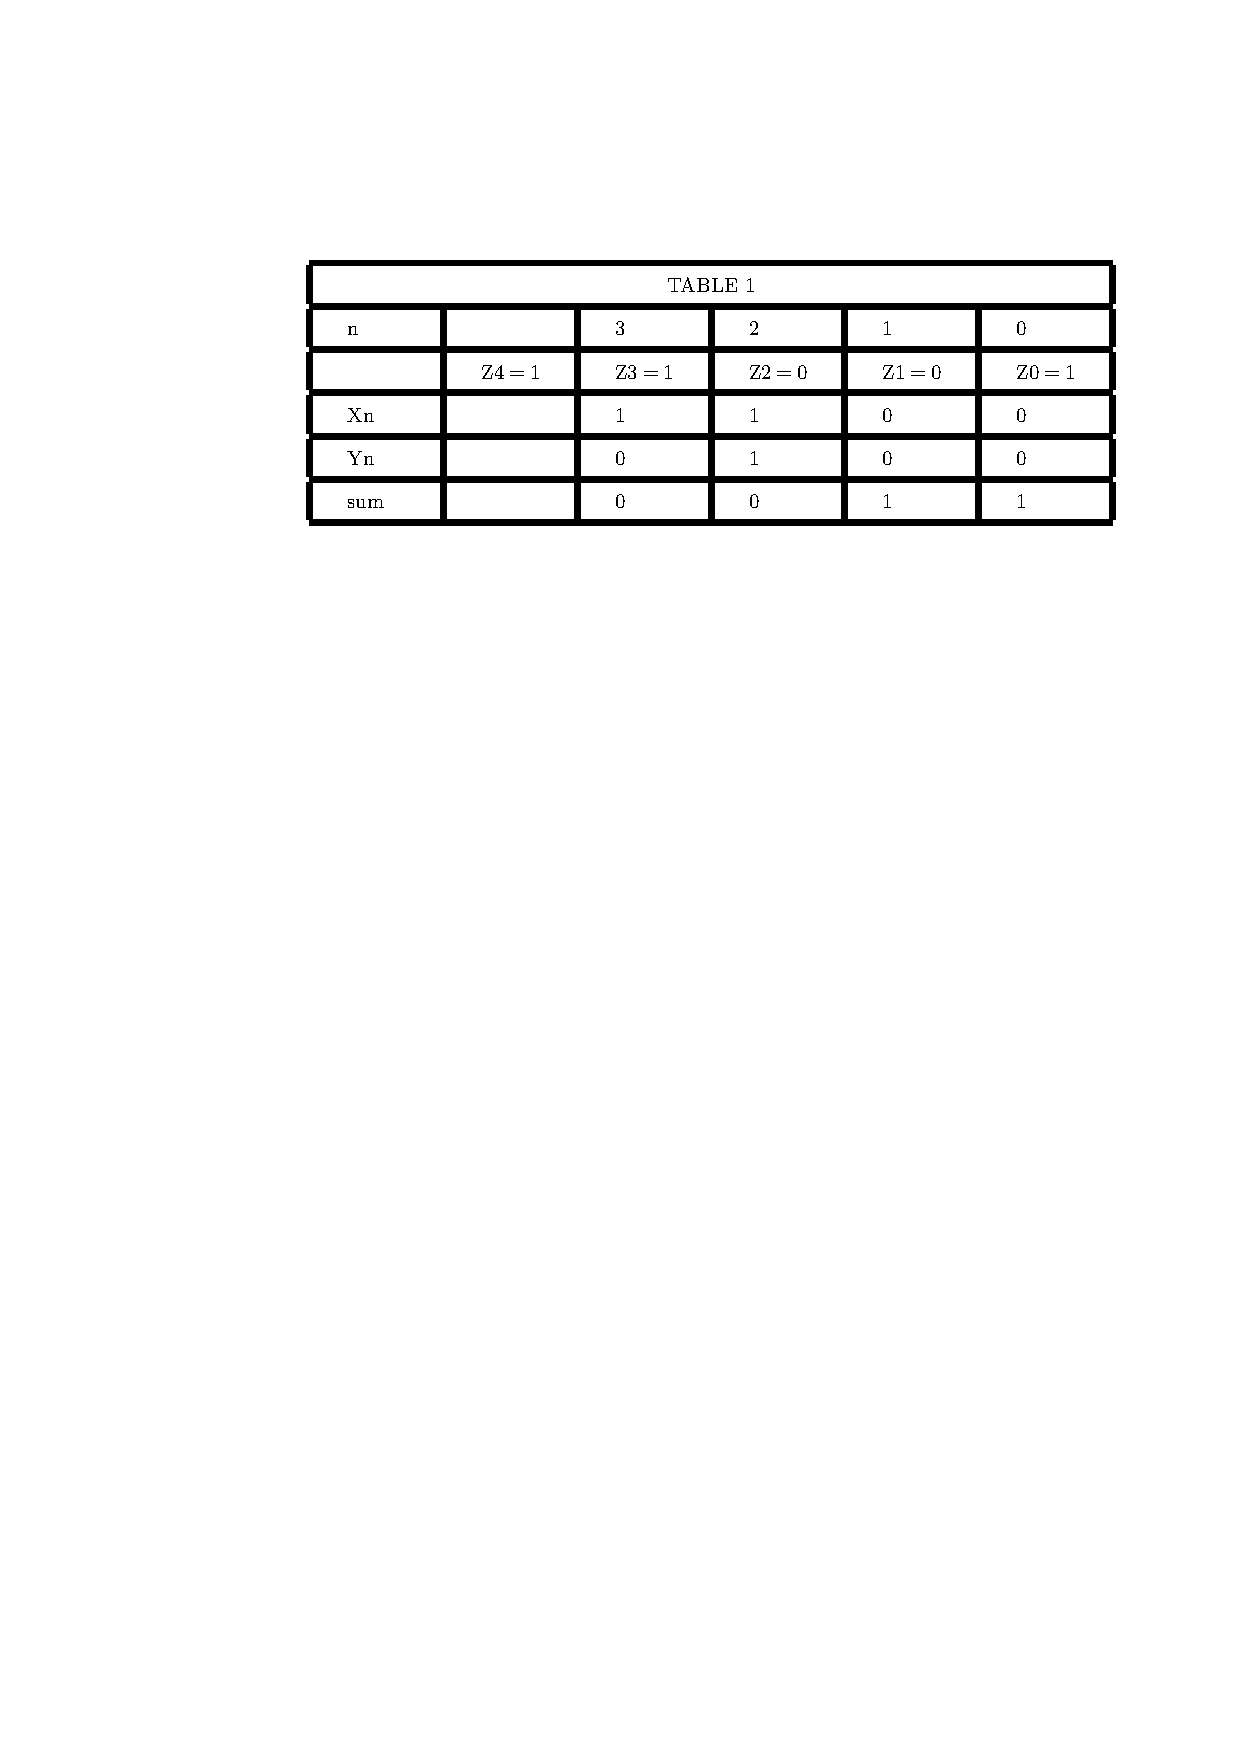
\includegraphics[scale=1.]{table.pdf}}
	
	\label{table.pdf}
\end{figure}
      

      



The delay in Z3 Output = (1)And+ (1)Or gate delay 
i.e 15 + 10 = 25 ns.



The delay in Z4 Output = delay in Z3 input + (1)And + (1)Or gate i.e 25 + 15 + 10 = 50 ns.        
 

So the output of the ripple carry adder will be stable at t = 50 ns.



(Full adder 1 is less significance so we did not considered that,and the reason why we did not considered XOR gate in figure 2  is because the delay of XOR gate is less than the delay of Z3 input i.e 20ns < 25ns ).



Hence the output of the ripple carry adder will be stable at t = 50 ns.


         
         \end{answer}
         


  

\end{document}
